\documentclass{article} 

\usepackage{graphicx}
\usepackage[colorlinks=true, allcolors=blue]{hyperref}

\newcommand{\ttt}[1]{\texttt{#1}}

\title{on-the-road-again} 
\author{Andrew Crofts, Ben Duchild, and Liam Strand} 

\date{April 29, 2022}

\begin{document}

\maketitle

\section{Final Design}

\noindent\makebox[\textwidth]{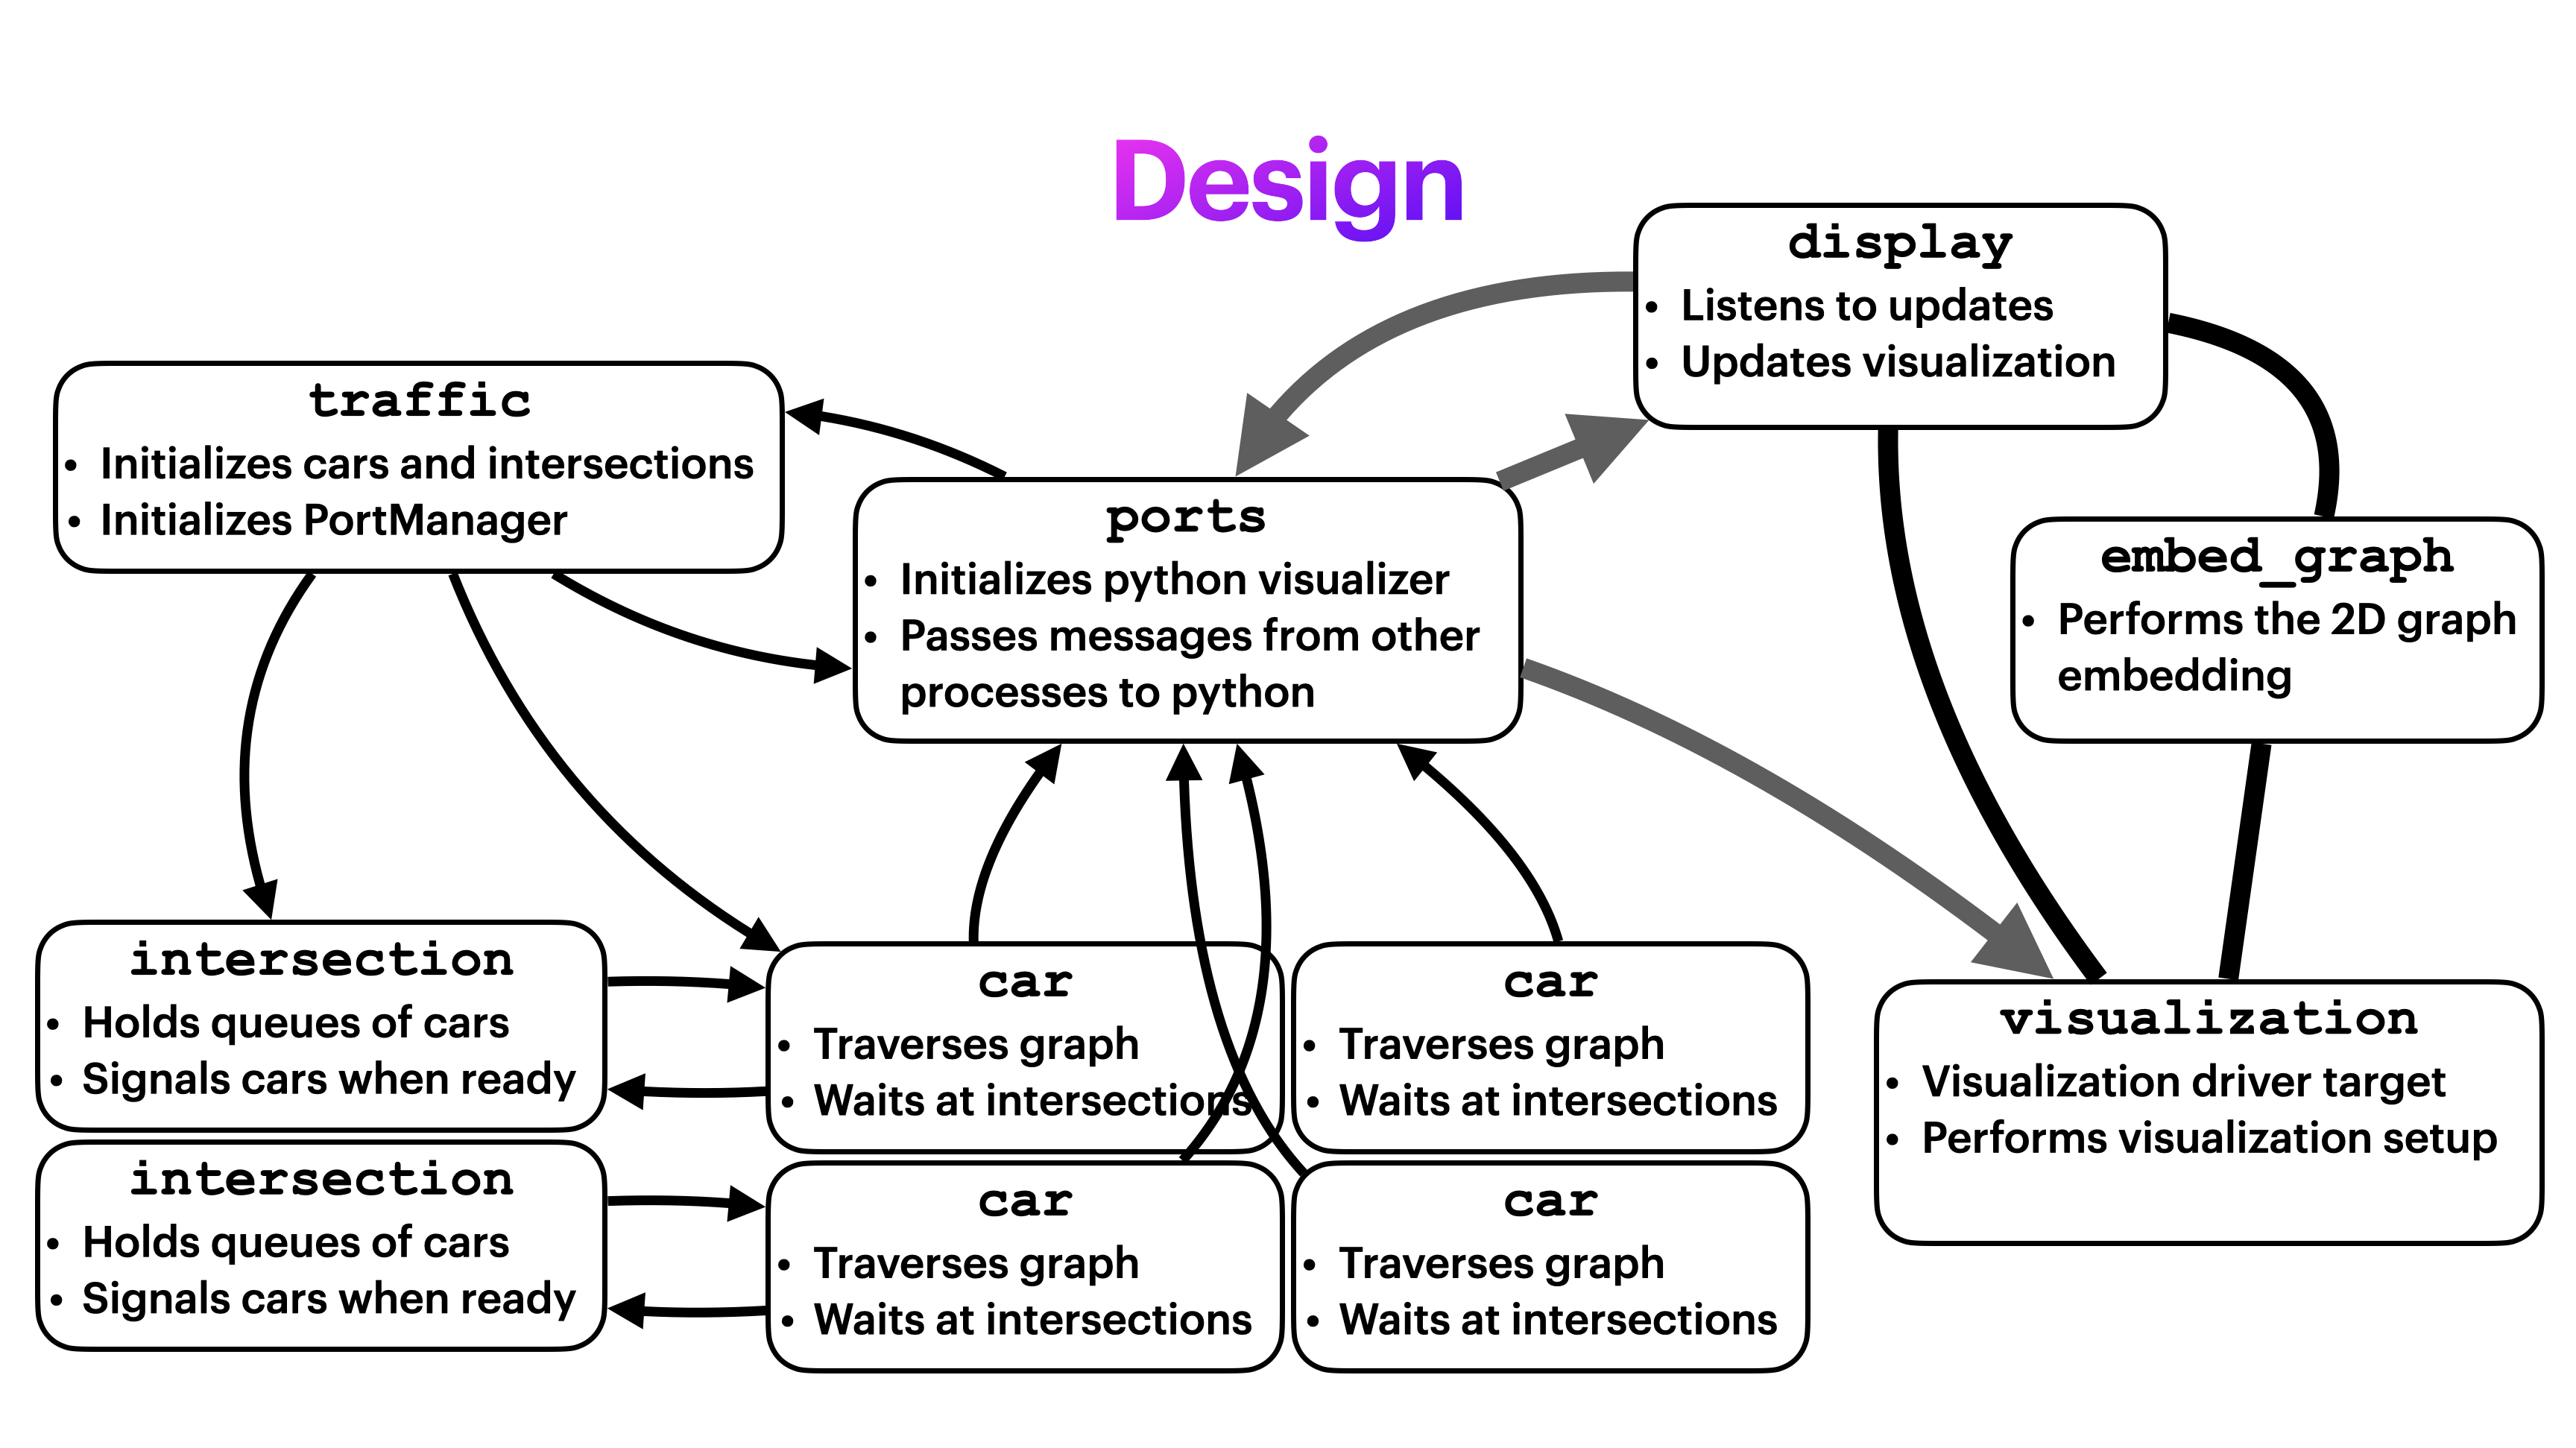
\includegraphics[width=\textwidth]{design-diagram.png}}

\noindent Changes from previous iteration:
\begin{itemize}
	\item Cars calculate their path at the very beginning of the simulation, rather than re-calculating at each intersection. We did this to improve performance.
	\item There are no records modeling roads; all roads have the same length, and are simply directed edges between intersections. We chose this to simplify the simulation, though it would be worthwhile to add more complex roads (different length/shape) if we had more time.
	\item We added a clock.erl module, which updates the visualization at a consistent pace, so the frontend can synchronize timing with the backend. 
	\item We added a ports.erl module, in order to abstract out communication with python and allow python to directly receive messages from a consistent process. 
	\item We reorganized the structure of the python side, because we didn't need to use inheritance as much as we expected. See later in this document for an overview of the python module structure.

\end{itemize}

\section{Outcome}

We achieved most of our minimum and maximum deliverables. Our program is general enough to simulate basic traffic networks (those which can be represented using a directed graph), but we failed to add in pedestrians. Once we implemented intersections and cars, it became apparent that adding pedestrians would make our problem much more difficult to solve: in order to have pedestrians, cars would need to communicate with pedestrians, and we would have to adopt a much more information-heavy spatial representation (something like Euclidean space, rather than a directed graph). 

Another complicating factor was that we weren't able to devote as much time to the project as we had hoped, because two team members were often preoccupied with comp 40 work.

\section{Reflection on Design}

\begin{itemize}
	\item Our best decision was to represent the roads using a digraph, because it made pathfinding, rendering, and configuration very simple. This decision did, however, complicate the visualization aspect of the project, as it was necessary to perform a 2D graph embedding to have something to draw.

	\item If we were to do this again, we would not split the program between Python and Erlang. Communication between the two languages proved to be very difficult, and the benefits of using Erlang actors did not outweigh the hassle.
\end{itemize}

\section{Design Decision}

We decided to represent a network of roads and intersections as a directed graph (roads are the edges, intersections are the nodes). Initially, we thought that a car's physical position on a road would be too difficult to simulate, so we decided it would be better if cars themselves just "jumped" between intersections after certain periods of time (which would correspond to speed and road length). 

Then, we thought about what part of the simulation would need to be concurrent, and figured out that it would be easiest for the cars to be concurrent, which would (practically speaking) require them to track their actual position on the road. We figured out that position tracking wouldn't be so difficult if we chose to model position as a value between 0 and 1, representing how far a car is along a given road. This seems like a good compromise between simplicity and realism.

\section{Devision of Labor}

Our division worked relatively well, although our roles often bled together at points when we had to synchronize and test our project. We found that a second (or third) set of eyes was always helpful when debugging.

\section{Development Timeline}

\begin{itemize}
	
	\item Week 0: Problem analysis, initial design, brainstorming, module/library exploration
	\item Week 1: Design refinement, first steps towards communication, problem simplification
	\item Week 2: First logical simulations, exploring other communication packages, first successful communication, lots of communication debugging
	\item Week 3: First visualization, vast visualization improvements, tune communication strategy
	\item Week 4: Buffered visualization with clock, visualization improvements, simulation tuning
	
\end{itemize}

\section{Bug Report}

Our toughest bug affected communication between Python and Erlang. We used Erlang Ports to facilitate communication between the two languages; the Erlang program launched a Python process, and received messages from it by reading from the python process’s stdout buffer. The documentation did not explicitly specify that stdout was used for communication, however. Our small Python-Erlang communication prototype worked as expected, but when we tried to add communication between Erlang and the pygame visualization, it simply didn't work. 

It took many hours over several days to debug. We had to examine the source code of the erlastic library, and figured out that stdout was used for communication. Even worse, the library gobbled everything from stdout, preventing us from seeing that there was erroneous data being sent through the Port. Things then became clear. On the Python side, we swapped \ttt{sys.stdout} and \ttt{sys.stderr}, and realized that pygame printed to stdout when it was imported. 

To solve this, then, we had to set an environment variable to silence pygame. Just to be safe, we also temporarily set \ttt{sys.stdout} to \ttt{sys.stderr} when we read in the digraph configuration, because the digraph layout library (grandalf) also echoed to stdout during the embedding.

\section{Instructions}

To run the program, simply navigate to the \ttt{build} directory and run \ttt{make}. The Makefile should handle all dependencies and then run the simulation, provided that the host system has recent versions of erlang and python3, as well as common lower-level libraries such as SDL2. 

\section{Overview of Code}

All code can be found in the \href{https://github.com/liam-strand/final-project}{GitHub repo}. The files written by us can be found in \ttt{src/}, with the exception of the \ttt{Makefile}, which is in \ttt{build/}.

\begin{itemize}

	\item \ttt{car.erl}
	\begin{itemize}
		\item an actor representation of a car; moves along roads, and contacts intersections along its route and waits to be signaled
		\item traffic.erl uses this module to launch car processes
	\end{itemize}
	\item \ttt{car.py}
	\begin{itemize}
		\item a very simple object-oriented representation of a car
		\item used by \ttt{display.py} to package together data about cars
	\end{itemize}
	\item \ttt{clock.erl}
	\begin{itemize}
		\item sends periodic messages to the python visualization
		\item used by \ttt{display.py} to synchronize with backend during idle time
	\end{itemize}
	\item \ttt{display.py}
	\begin{itemize}
		\item initializes visualization
		\item scales graph embedding to fit nicely on display
		\item handshakes with erlang to confirm connection
		\item listens to updates from erlang and modifies the displayed image to match
	\end{itemize}
	\item \ttt{embed\_graph.py}
	\begin{itemize}
		\item Performs graph embedding of the directed graph 
		\item exports a dictionary mapping intersections to points
	\end{itemize}
	\item \ttt{intersection.erl}
	\begin{itemize}
		\item actor representation of an intersection, which rotates through queues of waiting cars and signals them
		\item \ttt{traffic.erl} uses this module to launch intersection processes
	\end{itemize}
	\item \ttt{Makefile}
	\begin{itemize}
		\item rules to verify and install dependencies
		\item rules to run the simulation
		\item a rule to clean up build files
	\end{itemize}
	\item \ttt{ports.erl}
	\begin{itemize}
		\item contains tools for communicating with the python visualization
		\item used by car, intersection, and traffic modules to send updates to python
	\end{itemize}
	\item \ttt{sim\_state.py}
	\begin{itemize}
		\item a bloated monstrosity for passing the initial configuration from the toml file to the graph embedding algorithm.
		\item a class is not necessary here, but Liam wanted practice
	\end{itemize}
	\item \ttt{traffic.erl}
	\begin{itemize} 
		\item loads a road network from a TOML file and launches visualization, roads, and intersections
		\item gets run by the client to start everything off
	\end{itemize}
	\item \ttt{visualization.py}
	\begin{itemize}
		\item the visualization “driver”
		\item contains the target script that is evoked when the Erlang port is opened
	\end{itemize}
\end{itemize}


\end{document}
